\section{背景}
\begin{frame}{LD Cycleによる生体リズムの研究}
        \begin{block}{概日リズムの研究:LD Cycle}
          \begin{itemize}
            \item 常態的な時差ぼけや交代制勤務は、生活習慣病のリスクを高める.
            \item LD Cycleは生体リズムのモデルに用いられ,光と暗闇の情報が外力として系に加わる.
            \item 外力や各パラメータの設定により周期的・カオス的な振る舞いを持つ.
            \item 一般にカオスの予測は難しい.\begin{itemize}
              \item 初期値鋭敏性.
            \end{itemize}
          \end{itemize}
        \end{block}
      

      
        \begin{figure}
          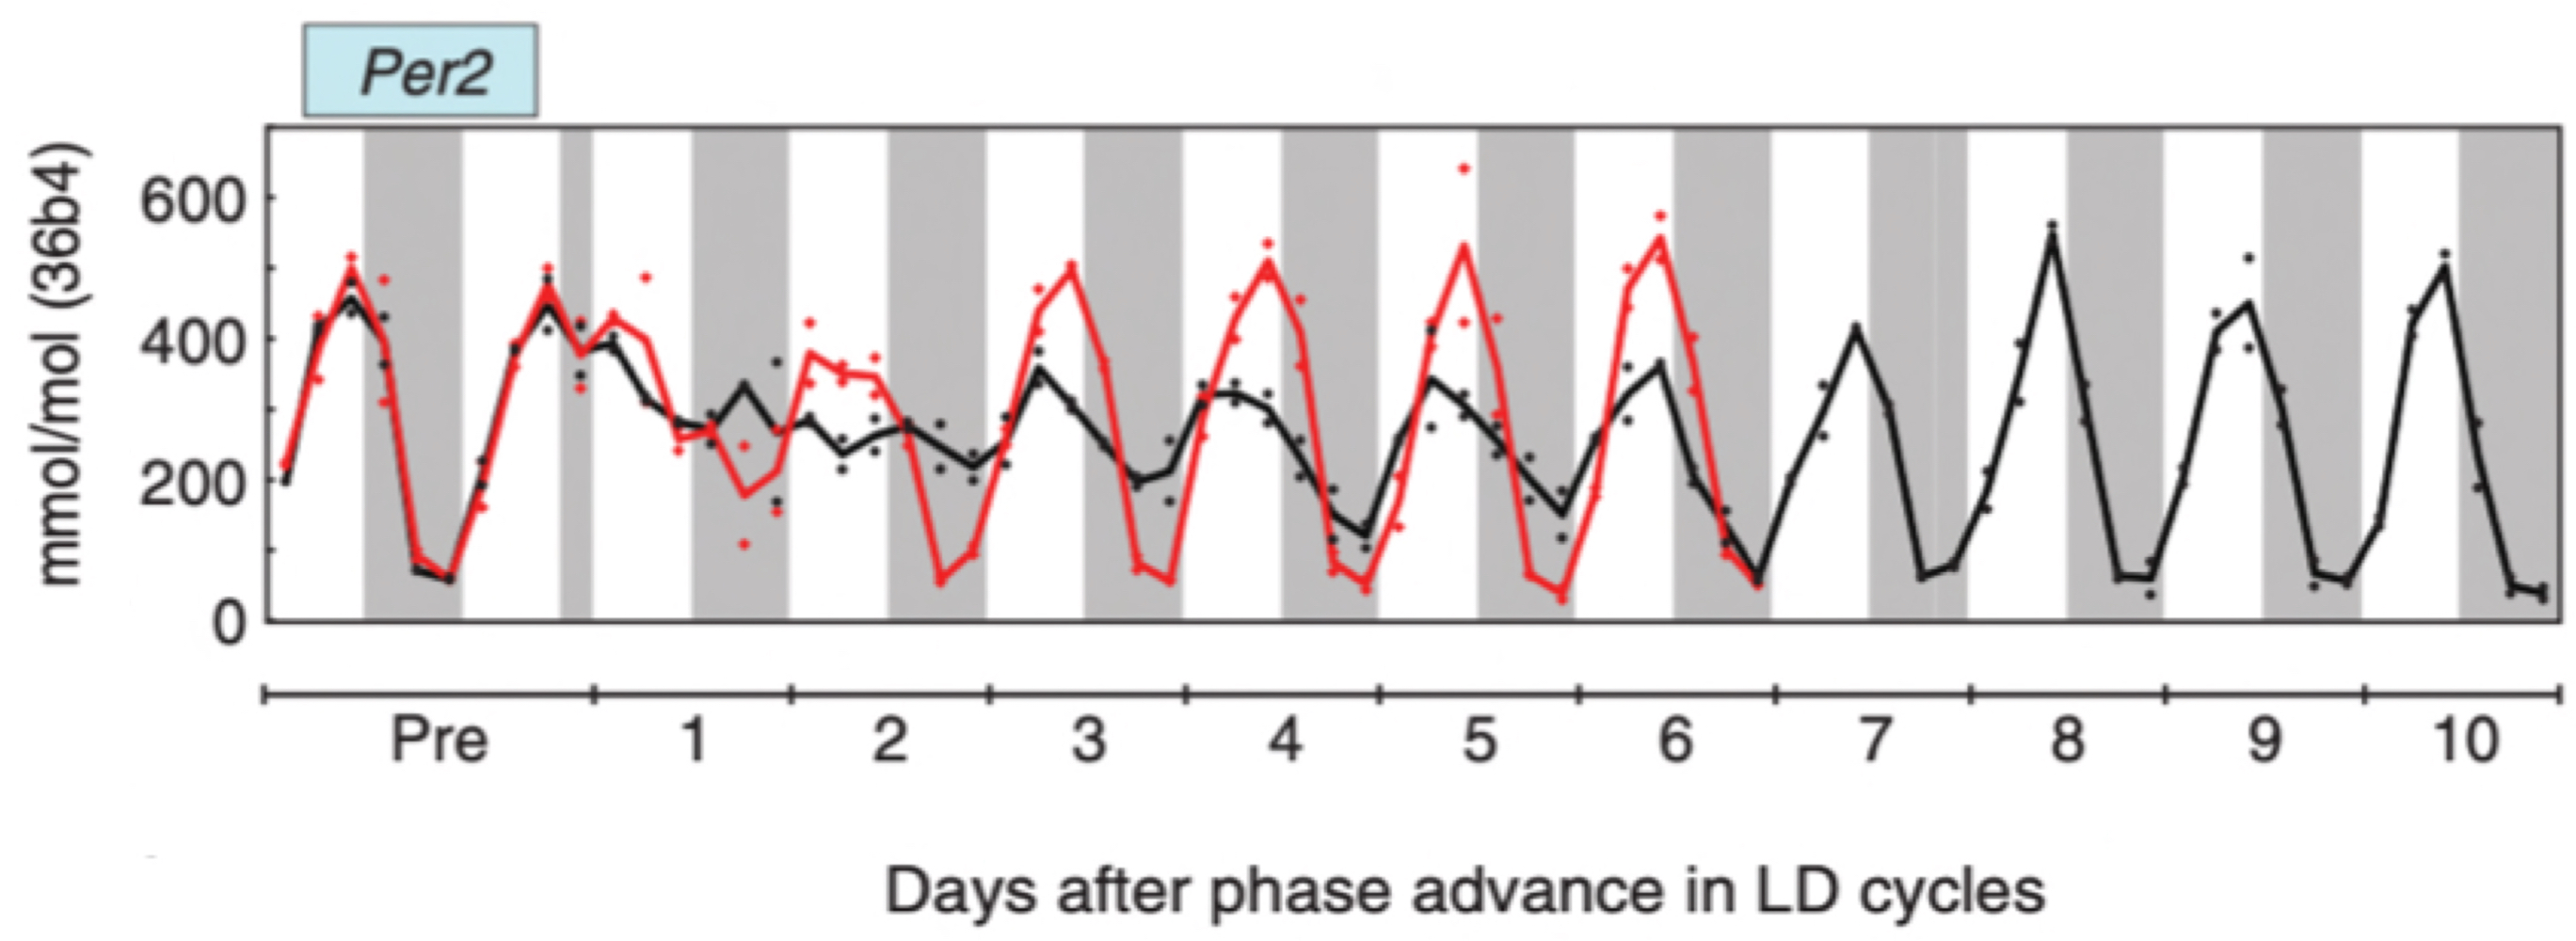
\includegraphics[width=0.4\textwidth]{Fig/Jetlag.png}
          \caption{\scriptsize{Day 1に8時間のJet Lagを受けた時のマウスの Per2 の推移}\\\tiny{Image: Fig.2 from \cite{Yamaguchi et al.}.}}
      \end{figure}    
      
  \end{frame}

  \section{手法}

\begin{frame}{Reservoir Computer を用いたカオス予測 (1/2)}
    % スライドを2つの列に分割
    \begin{columns}[T] % [T] は列を上部で揃えるオプション
  
      \begin{column}{.5\textwidth}
        
        \begin{itemize}
          \item 右側のアイテム1
          \item 右側のアイテム2
        \end{itemize}
      \end{column}

      \begin{column}{.5\textwidth}
        \begin{figure}
            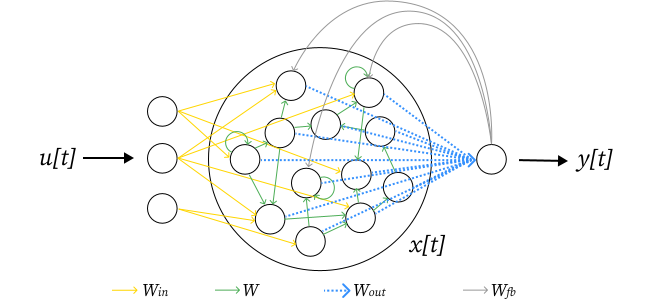
\includegraphics[width=\textwidth]{Fig/esn.svg.png}
        \end{figure}  
        \begin{figure}
            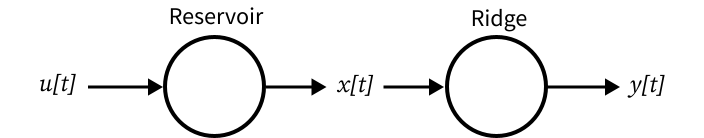
\includegraphics[width=\textwidth]{Fig/esn_nodes.svg.png}
            \caption{\scriptsize{Reservoirpy での reservoir computer の構造}\\ \tiny{Image: ReservoirPy, MIT License.}}
        \end{figure}  
      \end{column}
    \end{columns}
  \end{frame}


\begin{frame}{Reservoir Computer を用いたカオス予測 (2/2)}
% スライドを2つの列に分割
\begin{columns}[T] % [T] は列を上部で揃えるオプション

    \begin{column}{.5\textwidth}
    \vspace{-.35cm}
    % ここに右側のコンテンツを配置
    \begin{block}{予測の手法}
      \begin{enumerate}
        \item 予測する系の時系列データを生成\begin{itemize}
          \item 外力付きのRössler方程式の系の場合,変数 $X_t, Y_t$ と外力 $P_t$ から成る配列.
        \end{itemize}
        \item ReserviorのHyperparameterの最適化\begin{itemize}
          \item train 期間 で学習を行い,test期間で
          
          教師付きの予測を行う.
          \item test 期間での予測値と真の値との誤差を目的関数として,最適化を行う.
        \end{itemize}
        \item self-evolve 予測を行う.\begin{itemize}
          \item train, warm-up 期間 の後,
          Reservoir に未来予測をさせる.
          \item 各ステップの入力は,Reserviorの一期前の出力に対して,外力の真の値だけ
          
          修正した配列.
        \end{itemize}
    \end{enumerate}
    \end{block}
    \end{column}

    \begin{column}{.5\textwidth}
    \begin{figure}
        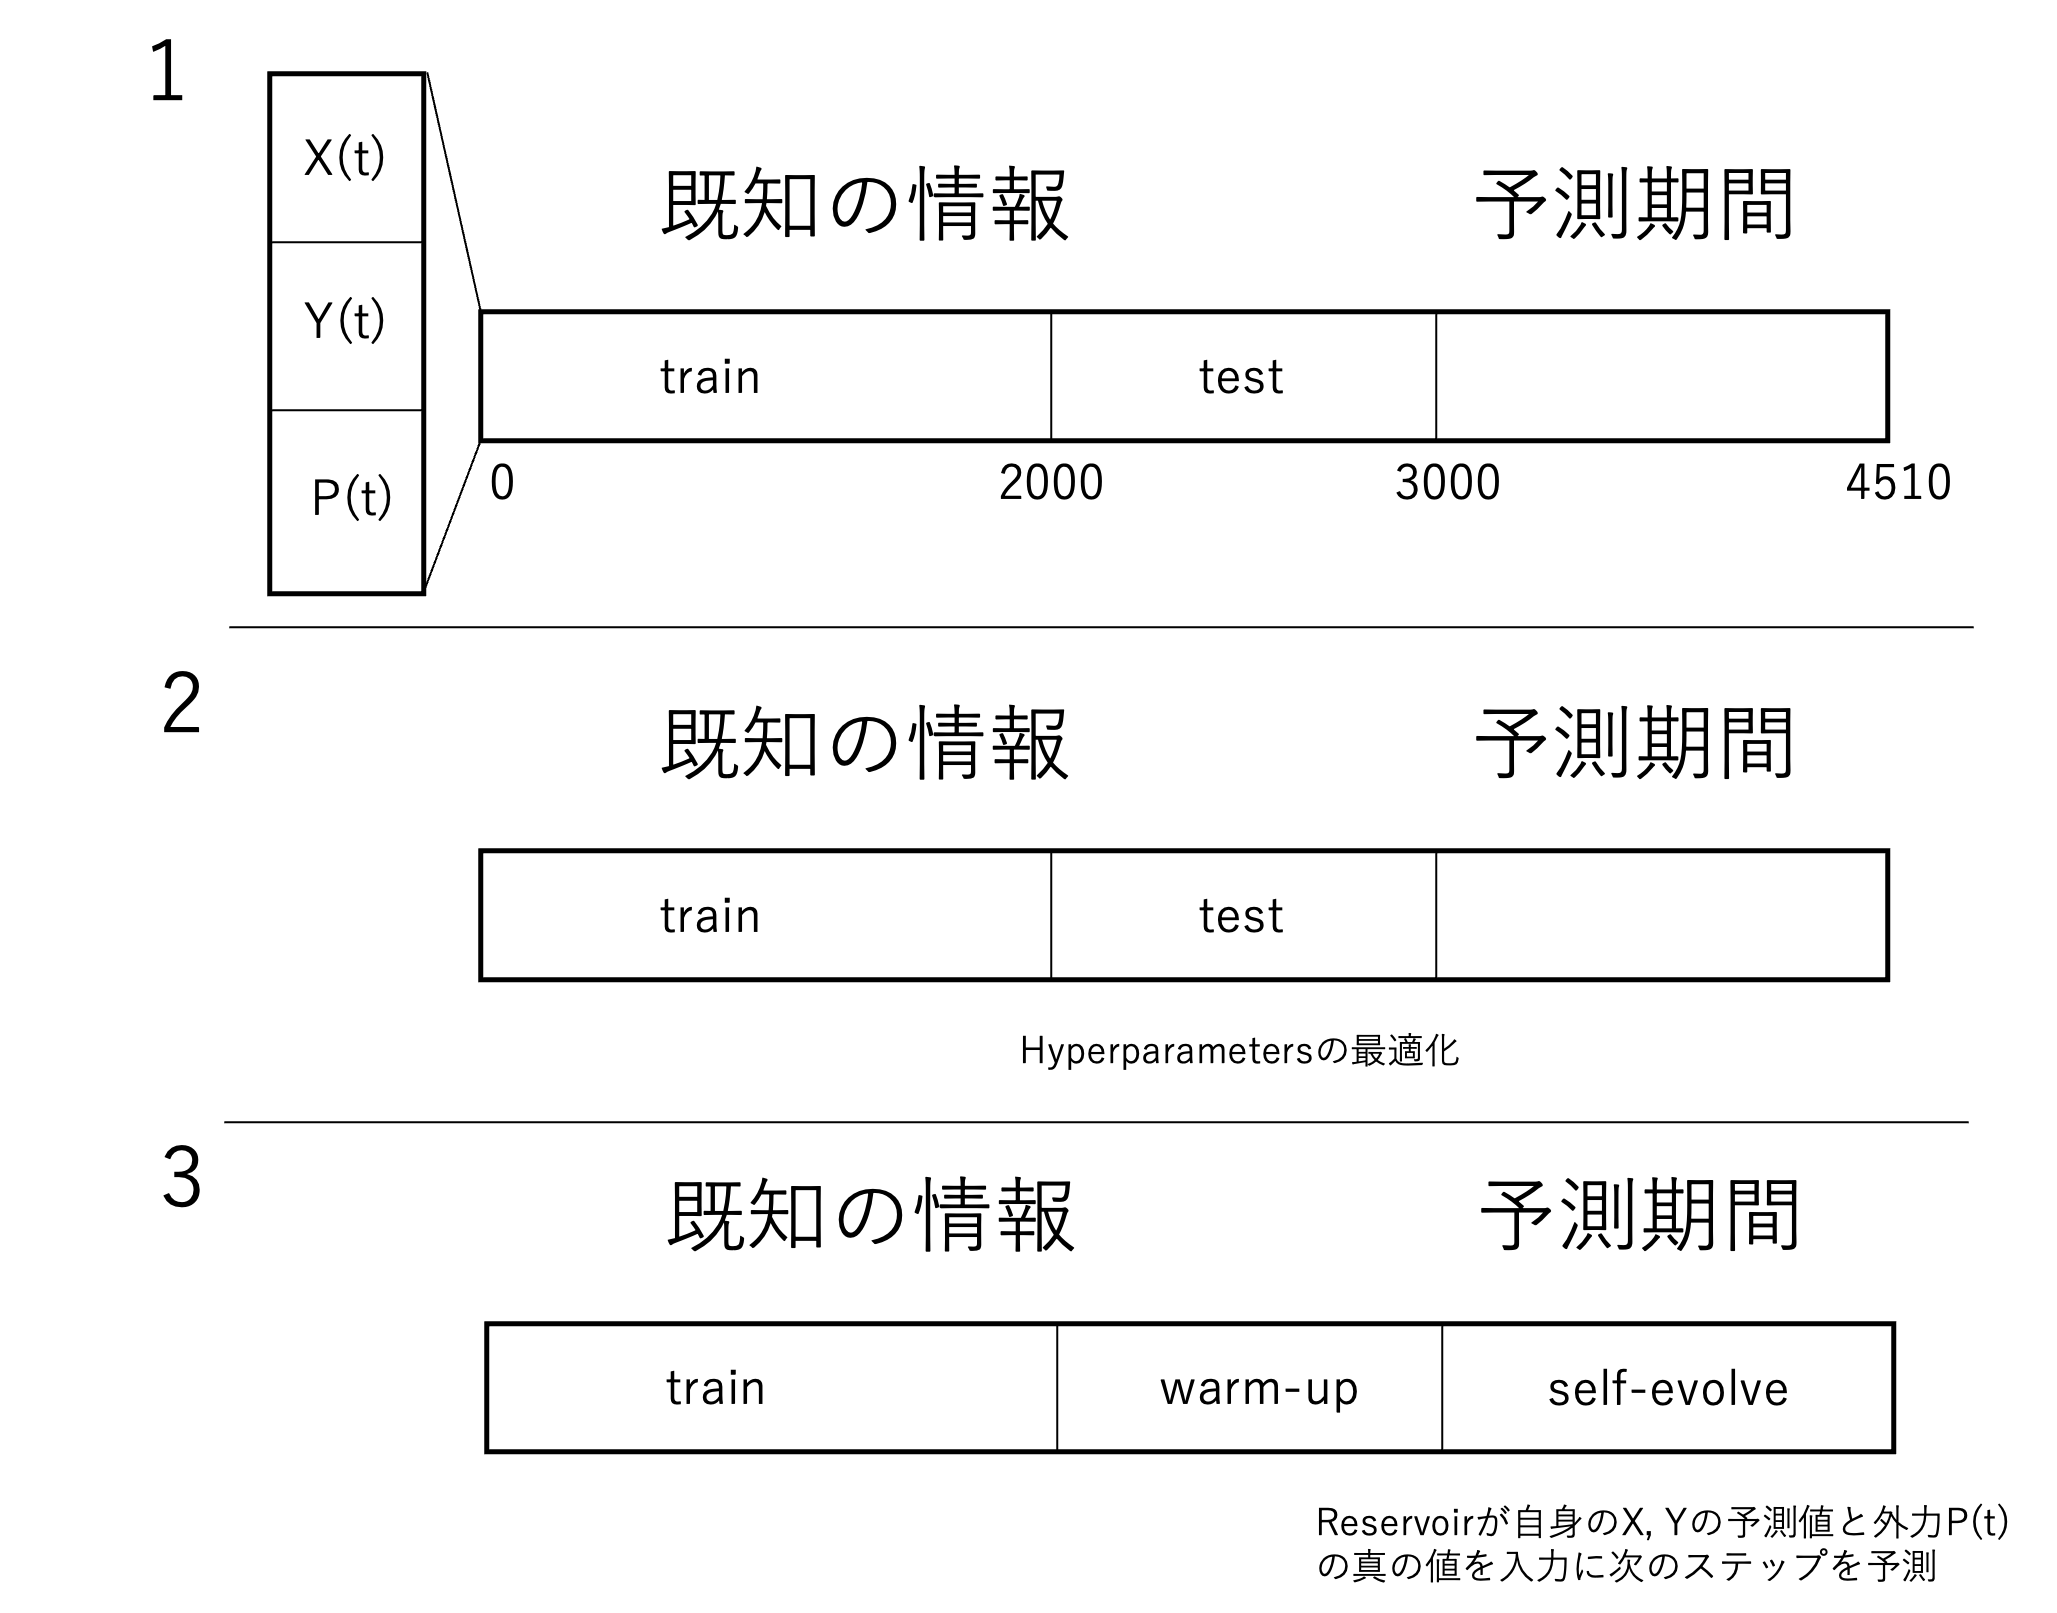
\includegraphics[width=\textwidth]{Fig/please.png}
        \caption{\scriptsize{Reservoir Computer を用いたカオス予測の手順}}
    \end{figure}   
    \end{column}
\end{columns}
\end{frame}
